
\subsection{The Jazz Influence Process over Time (Task~6)}\label{subsec:t6-jazz}

Task~6 asks for the influence process of musical evolution over time in one genre, for indicators
that reveal the dynamic influencers, and for an explanation of how the genre and its artists
changed. We study jazz. The choice continues \cref{subsec:q1-jazz}: the Jazz-induced subnetwork
there (384 artists, 1,769 edges) is the genre subnetwork examined in Model~I, and it spans the
whole record. It also gives the revolution windows of T5 (\cref{subsec:t5-revolutions}) a
genre-level test: the question is not only whether a decade is a revolution in the all-genre
catalogue, but which jazz artists moved, and whether their followers moved with them.

\paragraph{A release-year timeline.}
We use the same 42,770 edges as Model~I under Assumption~A3, including the 733 time-order
reversals. 406 artists carry the Jazz label; 384 of them form the both-endpoints-jazz
subnetwork of \cref{subsec:q1-jazz}. The Spotify files contain 8,000 jazz songs by
404 of these artists; 285 artists have at least three songs and can be given
a stable feature vector. Three clocks are kept separate: a song's release year \(y\), an artist's
active-start decade \(t_i\), and a follower's active-start decade (the cohort clock of
\cref{subsec:q1-cohorts}). The first describes the genre's sound, the second places an artist's
generation, and the third is used to validate transmission.

Model~II represents an artist by eleven Spotify coordinates (\cref{sec:model-similarity}); we use
its nine \emph{sound} coordinates, dropping \texttt{liveness} and \texttt{popularity}. Liveness
separates live from studio recordings --- a \(k\)-means run that includes it sets apart a
589-song cluster almost entirely by liveness ($+4.7$ standard deviations) --- and
popularity is not a property of the sound. All coordinates are \(z\)-scored across the artists of
\texttt{data\_by\_artist.csv}. This is a deliberate difference from T5, which uses all eleven
yearly aggregates and finds liveness the dominant 1970s driver; the robustness paragraph below
shows that adding liveness back changes the indicator rankings only marginally.

For each year with at least 20 jazz songs we compute the mean \(z\)-vector
\(\mathbf{x}_J(y)\), smooth it with a centred three-year window, and interpolate between years.
This leaves a reliable series from 1936 to 2002; earlier and later years are too sparse
for a yearly curve, and the 2010s (22 songs) are excluded from the decade summaries. A principal
component analysis of the yearly centroids gives PC1 59.3\% (acoustic and short recordings at
the positive end, long and electric ones at the negative end; loadings duration $-0.79$, acousticness $+0.52$, energy $-0.24$) and PC2
16.8\% (loadings instrumentalness $+0.58$, energy $+0.48$, valence $+0.42$). \cref{fig:t6-timeline} shows the decade trajectory and the
standardized decade centroids.

\begin{figure}[htbp]
\centering
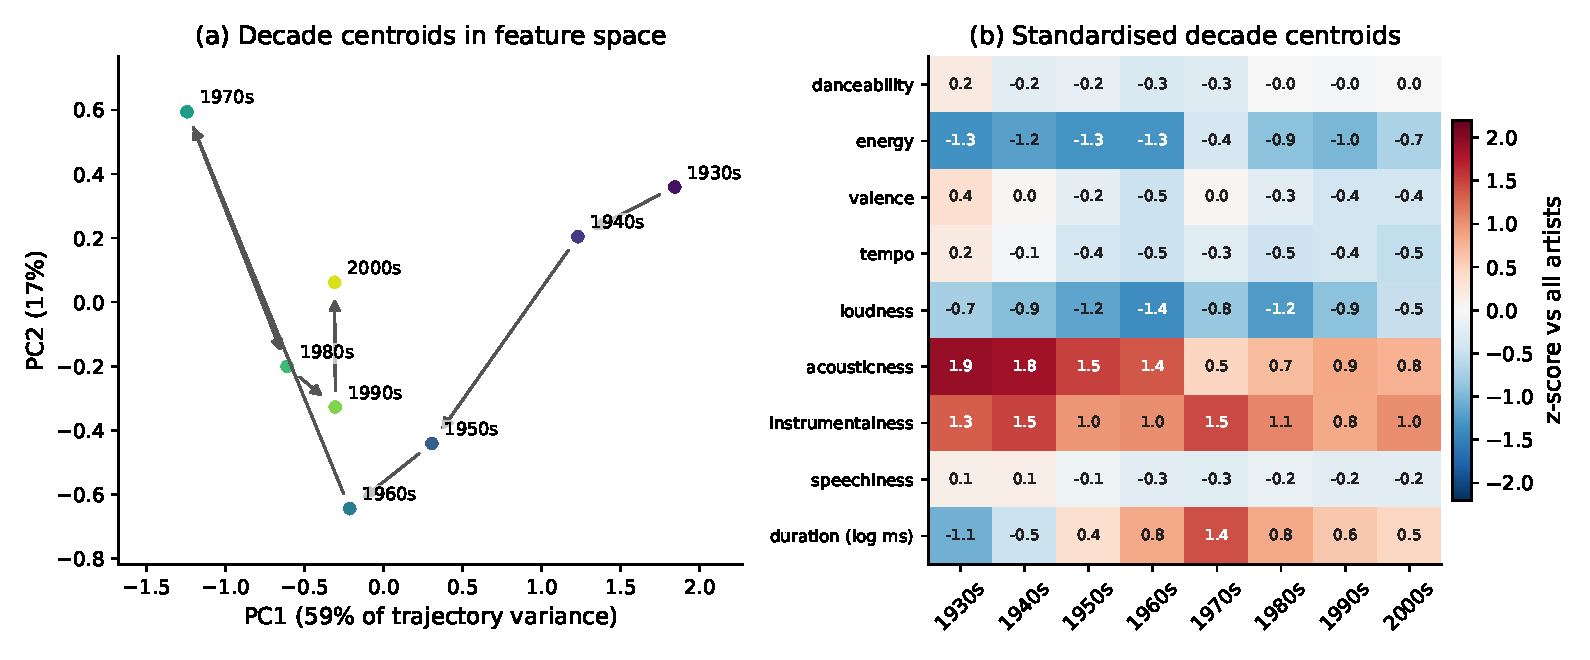
\includegraphics[width=\textwidth]{fig_t6_timeline.pdf}
\caption{Jazz sonic timeline. (a) Decade centroids in the first two principal components of the
yearly release-year centroids; arrows follow the decades. (b) Standardized decade centroids of the
nine sound features.}
\label{fig:t6-timeline}
\end{figure}

The trajectory is a loop. The 1930s centroid is the most acoustic and the shortest of the series
(acousticness 0.91, duration 3.0 min, tempo 124 BPM, valence
0.62); the 1950s--60s lengthen and darken; the 1970s is the most electric, highest-energy
and longest decade (acousticness 0.48, energy 0.51, duration 6.7 min); and
the 1980s--2000s recover part way towards an acoustic sound (0.55, 0.60,
0.57) without returning to the 1930s values.

\paragraph{Four jazz-specific episodes.}
The speed \(\|\mathbf{x}_J(y+2)-\mathbf{x}_J(y-2)\|\) has four well-separated local maxima, at
1949, 1954, 1969 and 1980 (\cref{fig:t6-episodes}). Their feature decompositions separate a stylistic break, a
format change, an electric turn and a crossover reversal:
\begin{itemize}[leftmargin=1.2em,itemsep=0.15em]
\item 1949: duration $-1.28$, loudness $-1.07$, energy $-1.00$ --- the small-group bebop break with swing;
\item 1954: duration $+1.58$, instrumentalness $-0.43$, valence $-0.18$ --- consistent with the LP replacing the 78-rpm single;
\item 1969: duration $+0.76$, energy $+0.56$, acousticness $-0.55$ --- fusion and electric instruments;
\item 1980: speechiness $+0.59$, loudness $-0.51$, valence $-0.51$ --- crossover, smooth jazz and the start of the acoustic revival.
\end{itemize}
The 1969 episode is the jazz face of T5's strong 1970s window (\cref{fig:t5-dual}), and the 1954
format shift corresponds to T5's network-only weak 1950s window. T5 reaches the 1970s through
liveness (a production shift); the jazz-only space reaches it through acousticness, energy and
duration (a style shift). The two readings are complementary.

\begin{figure}[htbp]
\centering
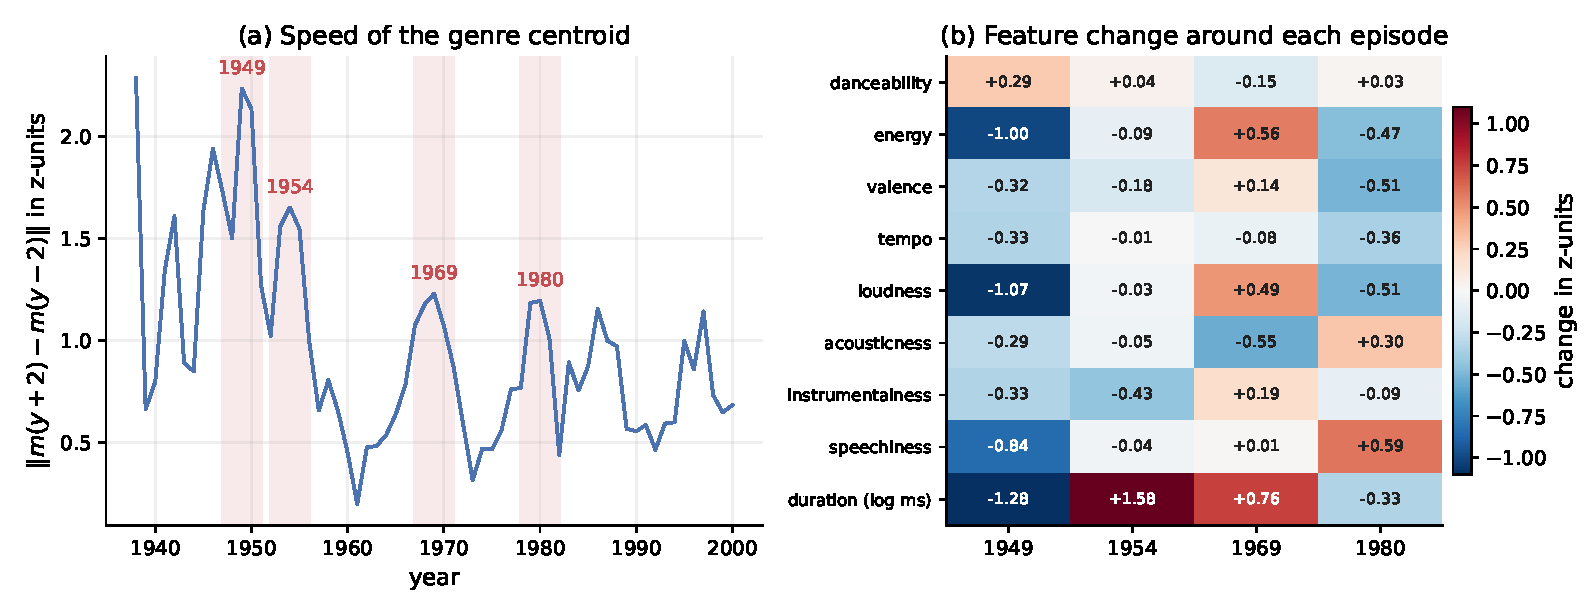
\includegraphics[width=\textwidth]{fig_t6_episodes.pdf}
\caption{Four jazz-specific episodes. (a) Speed of the jazz centroid; shaded bands mark the
episodes. (b) Change in each feature around each episode, $\mathbf{x}_J(y+2)-\mathbf{x}_J(y-2)$ in
\(z\)-units.}
\label{fig:t6-episodes}
\end{figure}

\paragraph{Indicators of dynamic influence.}
For artist \(i\) with \(n_i\ge3\) songs, let
\begin{equation}\label{eq:t6-r}
r_i=\frac{1}{n_i}\sum_{s\in i}\bigl(\tilde{\mathbf{x}}_s-\mathbf{x}_J(y_s)\bigr)
\end{equation}
be the \emph{time-adjusted deviation}: the average of the song vectors, each centred on the jazz
sound of its release year. The four indicators are:
\begin{align}
N_i&=\|r_i\|_\Sigma, \label{eq:t6-N}\\
A_i&=\cos(r_i,\Delta_i),\qquad \Delta_i=\mathbf{x}_J(t_i+10)-\mathbf{x}_J(t_i),
\label{eq:t6-A}\\
H_i&=\frac{1}{n_i^H}\sum_{j:\,i\to j,\ t_j>t_i}\cos(r_j,r_i),\qquad
H_i^*=H_i\,\frac{n_i^H}{n_i^H+3}, \label{eq:t6-H}
\end{align}
where \(N_i\) is originality (Mahalanobis length), \(A_i\) is anticipation (does the artist's
deviation point where the genre went over the next decade?), and \(H_i^*\) is transmission (did the
followers who name \(i\) move in \(i\)'s direction?), shrunk for small follower counts. Reach is
measured by \(K_i\), the within-jazz Katz score of \cref{subsec:q1-jazz}, and by \(B_i\), the number
of non-jazz followers; the Jazz$\to$Pop/Rock block alone contains 409 edges
(\cref{subsec:q3-inf-time}). The sonic indicators are defined for 283 artists; 175 have
a usable transmission score and 59 have at least five jazz followers.

\paragraph{Validation.}
There are 937 jazz$\to$jazz pairs with a later follower and at least three songs for both
artists. The mean alignment is 0.164. A within-decade permutation null (2{,}000 draws)
gives 0.024 \(\pm\) 0.030, so $p<0.001$; the bootstrap 95\% interval is
\([0.105,0.222]\). 56.4\% of the real pairs are positive against
51.2\% in the null. The effect is modest but real: reported influence is visible as a
small average movement of the follower's music in the influencer's direction. This complements the
matched-control similarity test of Task~4, which asks whether followers are closer to their
influencers than to controls; the present test asks whether they move \emph{towards} the
influencer's deviation from their own era.

The indicators are not redundant: \(N\)--\(A\) -0.02, \(N\)--\(K\) -0.37,
\(A\)--\(K\) +0.11, \(H^*\)--\(K\) +0.25. Originality is negatively related to citation
(-0.35 with future followers), anticipation is nearly independent of it (+0.09), and
transmission is the closest to future citation (+0.29). The most novel artists are not the
most cited, and being ahead is not the same as being central.

\paragraph{Dynamic influencers.}
We rank artists by \(S_i=z(A_i)+z(H_i^*)\), the equal-weight sum of the two standardized sonic
indicators, among the 59 artists with at least five jazz followers. Ranks are stable to
the weights (Spearman 0.910--0.979 for \(A\) weights 0.3--0.7) and to the transmission shrinkage
(raw and shrunk \(H\) correlate at 0.993). \cref{tab:t6-top} gives the top twelve;
\cref{fig:t6-influencers} maps anticipation against transmission.

\begin{table}[htbp]
\centering
\small
\caption{Top twelve dynamic influencers. \(N\) originality, \(A\) anticipation, \(H^*\)
transmission, ``Followers'' the number of usable jazz followers, \(K\) within-jazz Katz, \(B\)
non-jazz followers.}
\label{tab:t6-top}
\begin{tabular}{rlccccccc}
\toprule
\# & Artist & Start & \(N\) & \(A\) & \(H^*\) & Followers & \(K\) & \(B\) \\
\midrule
1 & Dave Brubeck & 1940s & 1.13 & +0.61 & +0.62 & 8 & 2.13 & 6 \\
2 & George Duke & 1960s & 1.62 & +0.36 & +0.66 & 5 & 1.69 & 10 \\
3 & Tal Farlow & 1940s & 2.46 & +0.92 & +0.38 & 8 & 3.03 & 2 \\
4 & Grover Washington, Jr. & 1960s & 1.19 & +0.23 & +0.70 & 8 & 2.32 & 1 \\
5 & David Sanborn & 1960s & 1.43 & +0.76 & +0.30 & 5 & 1.76 & 0 \\
6 & Bob James & 1960s & 1.76 & +0.30 & +0.50 & 6 & 1.77 & 2 \\
7 & Barney Kessel & 1940s & 3.38 & +0.69 & +0.23 & 6 & 4.81 & 2 \\
8 & Erroll Garner & 1940s & 2.18 & +0.74 & +0.20 & 11 & 4.52 & 4 \\
9 & Nat King Cole & 1930s & 2.31 & +0.54 & +0.27 & 11 & 5.07 & 52 \\
10 & Horace Silver & 1950s & 1.64 & +0.53 & +0.26 & 11 & 5.76 & 5 \\
11 & Oscar Peterson & 1940s & 2.44 & +0.79 & +0.12 & 14 & 4.66 & 4 \\
12 & Clifford Brown & 1950s & 1.42 & +0.69 & +0.15 & 6 & 3.13 & 0 \\
\bottomrule
\end{tabular}
\end{table}

\begin{figure}[htbp]
\centering
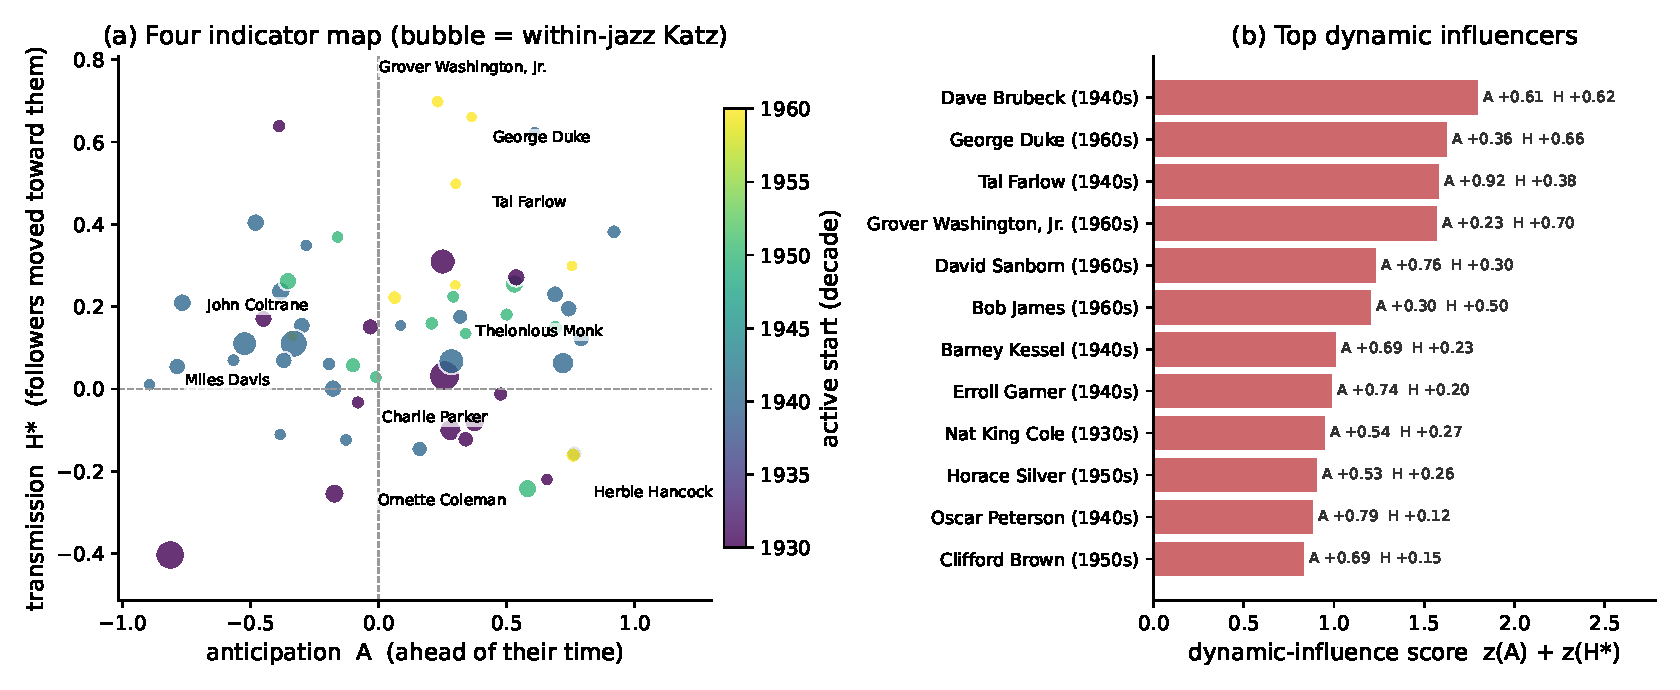
\includegraphics[width=\textwidth]{fig_t6_influencers.pdf}
\caption{(a) Anticipation against transmission for artists with at least five jazz followers;
bubble area is within-jazz Katz and colour is the active-start decade. (b) The top twelve by
\(S=z(A)+z(H^*)\), annotated with the two component scores.}
\label{fig:t6-influencers}
\end{figure}

\paragraph{Four roles.}
The \emph{canon} (high \(K\)) is Charlie Parker (17.2), Lester Young (15.5), Miles
Davis (13.9), Dizzy Gillespie, Thelonious Monk and John Coltrane (10.8). Their
anticipation is mixed and often negative, because they define the centre of their generation. The
\emph{catalysts} have high \(A\) and high \(H^*\): Dave Brubeck (+0.61/+0.62), George
Duke, Tal Farlow (+0.92), Grover Washington, Jr., David Sanborn and Bob James. The
\emph{prophets} are ahead but not copied: Duke Jordan, Shelly Manne, Jimmy Giuffre and John Lewis,
with Herbie Hancock (+0.76/-0.16), Lee Morgan and Andrew Hill in the 1960s
generation. The \emph{bridges} export influence beyond jazz: Miles Davis (77 non-jazz
followers), Nat King Cole (52), John Coltrane (52), Quincy Jones (25)
and Sun Ra (24).

\paragraph{How jazz changed.}
The swing baseline is acoustic and short (1930s: 0.91, 3.0 min, 124
BPM); Lester Young is the pure canon type ($K=15.5$, $A=-0.81$), and Cab Calloway is a
bridge (23 non-jazz followers). The 1949 bebop break
is visible in the cohort, not in Parker's distance from it: Parker has the highest within-jazz Katz
(17.2) but only $A=+0.26$ and $H^*=+0.03$; Bud Powell ($A=+0.72$) and
Gillespie ($H^*=+0.31$) carry more of the directional signal. The 1950s add the LP and
hard bop: Brubeck (+0.61/+0.62), Farlow ($A=+0.92$), Horace Silver
($A=+0.53$/$H^*=+0.26$) and Clifford Brown ($A=+0.69$). The late 1950s--60s
separate the canon from the avant-garde: Coltrane and Miles remain central ($K=10.8$
and 13.9) with negative anticipation, while Ornette Coleman
($A=+0.58$/$H^*=-0.24$, 16 non-jazz followers), Cecil Taylor
($A=+0.81$, $K=1.7$), Herbie Hancock ($A=+0.76$/$H^*=-0.16$) and
Andrew Hill ($A=+0.70$/$H^*=-0.31$) are ahead of the centre. The 1970s is fusion:
Hancock, Tony Williams ($A=+0.73$), John McLaughlin ($A=+0.38$/$H^*=+0.48$,
5 non-jazz followers) and Weather Report (10 non-jazz followers), with
Miles as the boundary bridge. The 1980s--2000s turn to crossover: George Duke
(+0.36/+0.66), Grover Washington, Jr. (+0.23/+0.70), Bob James
(+0.30/+0.50) and David Sanborn (+0.76/+0.30), with Wynton Marsalis
($A=+0.31$) marking the neoclassical reaction but having no usable jazz follower in this
edge set.

Across the period the influence process has two mechanisms. \emph{Canonical transmission}
reproduces the centre: the most cited artists define what the next generation sounds like, which
shows up as high \(K\) with low \(A\) and \(H^*\). \emph{Catalytic transmission} moves the centre: an
artist's deviation points where the genre goes and the followers move towards it, which shows up as
high \(A\) and \(H^*\). The largest movements occur when the second mechanism meets an opening that
is not itself musical --- the LP in the 1950s, electric instruments and amplification in the late
1960s, and multitrack production in the 1980s. This is also where the social and technological
dimension of the problem enters the network: it enters as a change of recording format and
production that shifts the feature centroid before the influence network catches up.

\paragraph{Limits and robustness.}
Only 285 of the 406 jazz artists have at least three songs, 175 have a usable
transmission score, and 59 have at least five followers; the ranking is therefore
descriptive rather than definitive. The 2010s (22 songs) are excluded; the 1920s contain only 9.
Active-start is a decade, it comes from AllMusic while the features come from Spotify, and a
song's year is its release year, not its composition year. Career averages are replaced by
song-level residuals, but the genre label remains coarse: ``Jazz'' covers swing, bebop, free jazz
and smooth jazz. Leave-one-out centroids change the originality and anticipation rankings by
Spearman 0.996 and 0.999; adding liveness gives 0.965 and 0.993; a five-year
anticipation horizon gives 0.766. The transmission test controls for decade composition but not
for shared scene or label, and it is an association between reported influence and sonic
direction, not a causal effect.
